\chapter{Metodología de la investigación}

\section{Enfoque, tipo y diseño de investigación}

\subsection{Enfoque de investigación}

La investigación tiene un enfoque cuantitativo: analiza datos numéricos de ocurrencias (coordenadas, fecha, turno) mediante procedimientos computacionales y pruebas estadísticas \citep{hernandez2018}.

\subsection{Tipo y alcance de la investigación}

Es de tipo aplicado, porque busca información útil para la gestión del serenazgo, y de alcance descriptivo e inferencial: describe la distribución espacial y temporal de las ocurrencias y contrasta si esa distribución difiere de la esperada por azar. No busca explicar causas.

\subsection{Diseño de investigación}

El diseño es no experimental y retrospectivo, con observaciones fechadas entre el 1 de enero y el 29 de agosto de 2025. No se manipula ninguna variable. El proceso de trabajo se alinea con las fases de CRISP-DM \citep{chapman2000}: comprensión de los datos, preparación, modelado, evaluación y comunicación de resultados (Figura~\ref{fig:flujo}).

\begin{figure}[H]
\centering
\begin{tikzpicture}[node distance=0.35cm, every node/.style={font=\footnotesize},
  caja/.style={draw, rounded corners, align=center, minimum width=2.0cm, minimum height=1.1cm},
  flecha/.style={-{Stealth}, thick}]
  \node[caja] (a) {Recolección\\de datos};
  \node[caja, right=of a] (b) {Depuración y\\georreferenc.};
  \node[caja, right=of b] (c) {Agrupamiento\\espacial};
  \node[caja, right=of c] (d) {Contraste\\y análisis\\temporal};
  \node[caja, right=of d] (e) {Mapas y\\validación};
  \draw[flecha] (a)--(b); \draw[flecha] (b)--(c); \draw[flecha] (c)--(d); \draw[flecha] (d)--(e);
\end{tikzpicture}
\caption{Etapas del procedimiento metodológico.}
\label{fig:flujo}
\fuente{Elaboración propia, a partir de las fases de CRISP-DM \citep{chapman2000}.}
\end{figure}

\section{Definiciones y variables}

\subsection{Definiciones operativas}

\begin{description}[leftmargin=0pt,labelindent=0pt,font=\bfseries]
\item[Ocurrencia de seguridad ciudadana:] hecho atendido y registrado por el patrullaje municipal e integrado (serenazgo y Patrullaje Local Integrado) en el SIPCOP-M. Incluye hechos de distinta naturaleza; no todos son delitos: el 34\,\% de los registros es ``exposición a peligro o abandono de personas'', que probablemente corresponde a asistencia. Se definen dos conjuntos de análisis: el \textbf{principal}, con todo el extracto depurado, y el de \textbf{presuntos delitos}, que excluye esa modalidad y conserva las ocurrencias presuntamente contra el patrimonio y contra la vida, el cuerpo y la salud (unos 430 de 996 registros). La clasificación de cada modalidad se confirmará con la municipalidad.
\item[Grupo espacial (clúster):] conjunto de ocurrencias que DBSCAN o HDBSCAN agrupan por densidad. Es un resultado del algoritmo y, por sí solo, no implica que la concentración sea significativa.
\item[Hotspot:] grupo espacial cuyo número de ocurrencias supera lo esperado bajo aleatoriedad espacial completa, según el contraste de la sección~\ref{sec:montecarlo}.
\end{description}

\subsection{Variables y operacionalización}

Se trata de un estudio observacional sin variable independiente ni dependiente en sentido experimental. Se miden cuatro grupos de resultados, uno por cada propósito del estudio (Tabla~\ref{tab:operacionalizacion}).

\begin{table}[H]
\centering
\caption{Operacionalización de los resultados medidos.}
\label{tab:operacionalizacion}
\begingroup\singlespacing\footnotesize
\begin{tabular}{@{}p{2.5cm}p{2.6cm}p{5.4cm}p{2.9cm}@{}}
\toprule
\textbf{Objetivo} & \textbf{Dimensión} & \textbf{Indicadores} & \textbf{Instrumento} \\
\midrule
OE1 & Calidad de los registros & Porcentaje de registros utilizables; duplicados; datos incompletos o fuera del distrito & Base del SIPCOP-M; registro de depuración \\
\addlinespace
OE2 & Concentración espacial & Número y tamaño de los grupos; porcentaje de ruido; valor $p$ por grupo (Monte Carlo); silueta & DBSCAN; simulación en el polígono del distrito \\
\addlinespace
OE2 & Comparación de algoritmos & Índice de Rand ajustado entre asignaciones; número de grupos y ruido; estabilidad ante cambios de parámetros & DBSCAN y HDBSCAN \\
\addlinespace
OE3 & Comportamiento temporal & Frecuencias por turno, día de la semana y mes; $\chi^2$, valor $p$ ajustado y $V$ de Cramér & Base del SIPCOP-M; pruebas estadísticas \\
\bottomrule
\end{tabular}
\endgroup
\fuente{Elaboración propia.}
\end{table}

\section{Unidad de análisis, población y muestra}

\subsection{Unidad de análisis}

La unidad de análisis es la ocurrencia de seguridad ciudadana registrada en el SIPCOP-M, con su fecha, turno, tipo y ubicación. Los registros no tienen identificador único.

\subsection{Población y muestra}

La población accesible para este estudio está constituida por los 996 registros del extracto descargado de la capa SIPCOP Municipal, todos con \texttt{id\_dist=080105} y fecha de alerta entre el 1 de enero y el 29 de agosto de 2025. Se realizará un censo de ese extracto, no una muestra probabilística. Este total describe el archivo disponible y no se interpreta como la totalidad de las ocurrencias realmente atendidas por el serenazgo.

\textbf{Criterios de inclusión:} registros dentro del periodo, con fecha, turno, categoría y coordenadas utilizables, y cuya ubicación corresponda al distrito tras validar el sistema de referencia. \textbf{Criterios de exclusión:} duplicados exactos (filas idénticas en los 19 campos; son 10, con lo que 996 pasa a 986), registros sin campos esenciales o con coordenadas fuera del distrito. Como el archivo carece de identificador, los 70 registros con igual fecha, turno y coordenadas (``casi duplicados'') no se eliminan, porque pueden ser hechos distintos en puntos recurrentes; se evalúa su efecto en el análisis de sensibilidad. El número de registros excluidos por cada criterio se informará (Anexo~\ref{anx:depuracion}).

\subsection{Diagnóstico preliminar del extracto}

Antes del análisis se revisó el archivo descargado (Tabla~\ref{tab:diagnostico}). Este diagnóstico no contrasta ninguna hipótesis; sirve para fijar los parámetros del diseño con criterios explícitos.

\begin{table}[H]
\centering
\caption{Diagnóstico preliminar del extracto SIPCOP Municipal de San Sebastián.}
\label{tab:diagnostico}
\begingroup\singlespacing\footnotesize
\begin{tabular}{@{}p{4.4cm}p{9.6cm}@{}}
\toprule
\textbf{Aspecto} & \textbf{Hallazgo} \\
\midrule
Registros y periodo & 996 filas, 19 columnas; 1/1--29/8/2025 (241 días, 215 con registro y 26 sin ningún registro) \\
\addlinespace
Resolución espacial & Coordenadas en grados decimales con 3 decimales (unos 108 m en $x$ y 111 m en $y$); 412 ubicaciones distintas; 765 registros (77\,\%) comparten coordenada exacta con otro \\
\addlinespace
Duplicados & 10 filas idénticas; 70 con igual fecha, turno y coordenadas; sin identificador único \\
\addlinespace
Volumen mensual & Registros por día: 4,9 (ene.), 5,0 (feb.), 3,1 (mar.), 4,2 (abr.), 3,1 (may.), 2,0 (jun.), 3,5 (jul.) y 7,5 (ago., hasta el 29) \\
\addlinespace
Cambio de clasificación & Exposición a peligro o abandono: 339 registros (34\,\%); 57\,\% de los registros de enero y 9--17\,\% de junio a agosto \\
\addlinespace
Origen del registro & Patrullaje 760 (76\,\%); teléfono 216, alarma 13, mensajería 3; cámara, operativo y otros 4 \\
\addlinespace
Personal & Patrullaje Local Integrado 504 (51\,\%); Patrullaje Municipal -- Serenazgo 492 \\
\addlinespace
Campos esenciales & \texttt{fechaalerta}, \texttt{turno}, \texttt{especifico}, \texttt{modalidad}, \texttt{x} e \texttt{y} sin valores nulos \\
\addlinespace
Campos incompletos & \texttt{lugarocurrencia} 22\,\% faltante; \texttt{resultadoocurrencia} 67\,\% (casi solo en hechos contra la vida, el cuerpo y la salud); \texttt{consecuencia} 10\,\%; \texttt{medioutilizado} 32\,\% faltante y 64\,\% ``OTROS'' \\
\addlinespace
Campos constantes & \texttt{generico}, \texttt{estado} e \texttt{id\_dist} \\
\bottomrule
\end{tabular}
\endgroup
\fuente{Elaboración propia a partir del CSV SIPCOP Municipal (separador \texttt{;}, UTF-8 con BOM, fechas en texto en español, por ejemplo ``agosto 23, 2025'').}
\end{table}

La Figura~\ref{fig:ubicaciones} muestra las 412 ubicaciones distintas: se concentran en dos franjas este--oeste y varias repiten la misma coordenada, lo que es coherente con una geocodificación por puntos de referencia. La Figura~\ref{fig:mensual} muestra que el volumen de registro y la proporción de la modalidad de exposición a peligro o abandono cambian entre meses. Ambas figuras son descriptivas y orientan la elección del radio $\varepsilon$ y de la referencia temporal; no constituyen evidencia de concentración ni de patrón temporal alguno.

\begin{figure}[H]
\centering
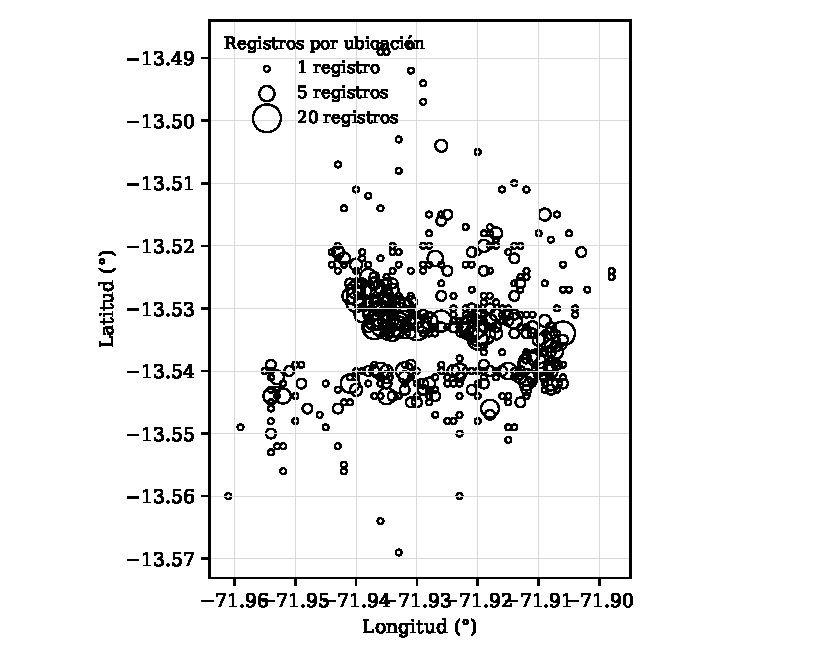
\includegraphics[width=0.72\textwidth]{diag_ubicaciones.pdf}
\caption{Ubicaciones distintas del extracto SIPCOP Municipal (San Sebastián, 2025).}
\label{fig:ubicaciones}
\fuente{Elaboración propia a partir del CSV SIPCOP Municipal. El tamaño del círculo es proporcional al número de registros con esa coordenada; $n = 996$ registros en 412 ubicaciones. Generada con \texttt{datos/figuras\_diagnostico.py}.}
\end{figure}

\begin{figure}[H]
\centering
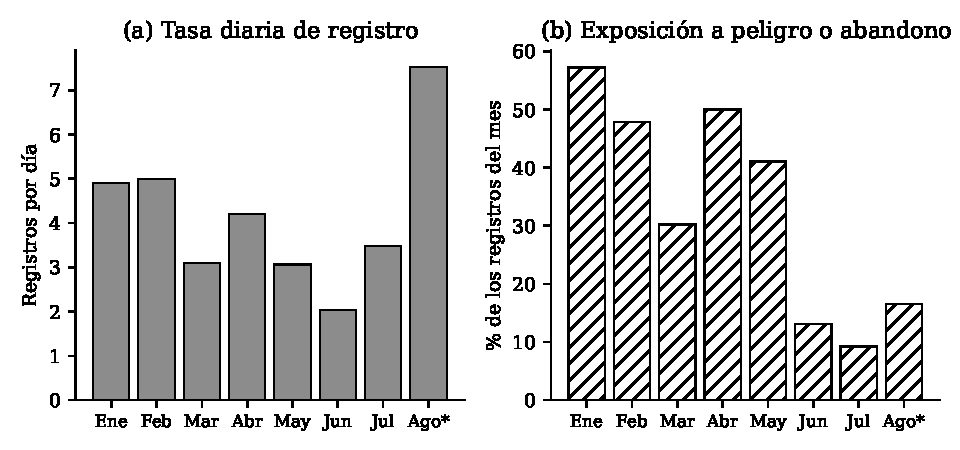
\includegraphics[width=0.95\textwidth]{diag_mensual.pdf}
\caption{Volumen de registro y modalidad de exposición a peligro o abandono por mes.}
\label{fig:mensual}
\fuente{Elaboración propia a partir del CSV SIPCOP Municipal. (*) Agosto incluye solo hasta el 29. En (a), la tasa es el número de registros dividido entre los días del mes observados; en (b), el porcentaje se calcula sobre los registros de cada mes.}
\end{figure}

\section{Técnicas e instrumentos de recolección}

\begin{itemize}
    \item \textbf{Análisis documental:} revisión del archivo CSV público de la capa SIPCOP Municipal para el distrito \texttt{080105}; se conservarán la URL de origen, fecha de descarga y archivo original para trazabilidad. Se solicitará a la municipalidad o al responsable de la capa la definición de los campos y del sistema de referencia espacial.
    \item \textbf{Instrumento:} ficha de estructura de datos (Anexo~\ref{anx:ficha}), que documenta las 19 columnas del archivo. Los campos analíticos son \texttt{fechaalerta}, \texttt{turno}, \texttt{especifico}, \texttt{modalidad}, \texttt{x} e \texttt{y}; se usan además \texttt{origen}, \texttt{naturalezadelpersonal}, \texttt{lugarocurrencia}, \texttt{consecuencia}, \texttt{formapatrullaje}, \texttt{direccion} y \texttt{tipovia} para la calidad de datos y los análisis de sensibilidad. El archivo no contiene una hora individual del hecho.
    \item \textbf{Cartografía:} polígono oficial del distrito y, si está disponible, la capa de manzanas o vías, para delimitar el área de simulación.
    \item \textbf{Herramientas de análisis:} Python con las bibliotecas \textit{pandas}, \textit{scikit-learn} \citep{pedregosa2011}, \textit{hdbscan} \citep{mcinnes2017} y \textit{SciPy}; un sistema de información geográfica para los mapas.
\end{itemize}

\section{Procedimiento metodológico}

\begin{enumerate}
    \item \textbf{Obtención y documentación.} Preservación del CSV disponible (996 registros; \texttt{id\_dist=080105}) y registro de su procedencia. Se consultará el significado de \texttt{fechaalerta}, los horarios de turno, las definiciones de categoría y la confirmación del sistema de referencia (el diagnóstico indica longitud y latitud en grados decimales, WGS84); cualquier autorización o validación municipal necesaria se gestionará antes de difundir resultados.
    \item \textbf{Depuración.} Revisión de duplicados, parseo de fechas, normalización de turnos y categorías, y comprobación de que las coordenadas correspondan al distrito. Se calculará la proporción de registros utilizables (objetivo específico~1) y se documentarán exclusiones.
    \item \textbf{Validación espacial.} Se verificará que \texttt{x} sea longitud e \texttt{y} latitud y que el sistema de referencia sea WGS84. Además se revisarán tres aspectos: (i) la cuantización a 0,001° y los ceros finales omitidos (126 valores de \texttt{x} y 145 de \texttt{y} tienen solo dos decimales); (ii) el contraste entre \texttt{direccion} y las coordenadas, usando puntos de referencia reconocibles (paraderos, el cementerio, el centro de salud); y (iii) la superposición con el polígono oficial del distrito. Solo después se transformarán a un sistema proyectado métrico o se usará haversine; si no se logra confirmar la referencia, no se interpretarán distancias ni agrupamientos métricos.
    \item \textbf{Análisis exploratorio.} Series por mes, día de la semana y turno dentro del periodo disponible; mapa de puntos y de densidad kernel (solo como visualización).
    \item \textbf{Agrupamiento espacial.} Se aplica DBSCAN con distancia haversine (Algoritmo~\ref{alg:dbscan}) y se elige la configuración según la regla de la sección~\ref{sec:parametros}. HDBSCAN se ejecuta como comparación.
    \item \textbf{Contraste de la concentración espacial.} Prueba Monte Carlo por grupo frente a aleatoriedad espacial completa (sección~\ref{sec:montecarlo}); los grupos significativos son los \textit{hotspots}.
    \item \textbf{Análisis temporal de los \textit{hotspots}.} Contrastes chi-cuadrado por turno, día de la semana y mes (sección~\ref{sec:temporal}).
    \item \textbf{Validación y presentación.} Revisión de los \textit{hotspots} con el personal del patrullaje municipal y elaboración de mapas.
\end{enumerate}

\algtitulo{DBSCAN aplicado a las ocurrencias georreferenciadas.}\label{alg:dbscan}
\noindent\textbf{Algoritmo \thealgoritmo.} DBSCAN aplicado a las ocurrencias georreferenciadas.
\begin{enumerate}
  \item Inicializar $C \gets 0$ y marcar todos los puntos como no visitados.
  \item Para cada punto $p \in D$ no visitado: marcarlo como visitado y calcular su vecindario $N_{\varepsilon}(p)$ con la distancia $d$ (ecuación~\ref{eq:haversine}).
  \item Si $|N_{\varepsilon}(p)| < \mathrm{MinPts}$, etiquetar $p$ como ruido.
  \item En caso contrario, crear un nuevo grupo $C$, asignar $p$ a dicho grupo y expandirlo con todos los puntos alcanzables dentro del radio $\varepsilon$.
  \item Repetir hasta que todos los puntos queden etiquetados como pertenecientes a un grupo o como ruido.
\end{enumerate}

\section{Protocolo de evaluación}

\subsection{Selección de parámetros y calidad del agrupamiento}
\label{sec:parametros}

La regla de selección se fija antes de ver los resultados de los contrastes. Las coordenadas tienen resolución de 0,001° (unos 108--111 m): dos puntos de celdas distintas distan al menos ese paso, de modo que con $\varepsilon \leq 100$ m solo se agrupan registros con coordenada idéntica, y $\varepsilon = 50$ y $100$ m producen la misma partición (diagnóstico preliminar). Por ello se explora una rejilla de $\varepsilon \in \{150, 200, 250, 300\}$ m y $\mathrm{MinPts} \in \{10, 20, 30\}$, y el gráfico de $k$-distancias orienta el rango de $\varepsilon$. Los registros con coordenadas idénticas cuentan como puntos separados al evaluar MinPts. Para cada configuración se calculan el número de grupos, el porcentaje de ruido y la silueta media (ecuación~\ref{eq:silueta}) sobre los puntos asignados. Se elige la configuración con mayor estabilidad, medida como el índice de Rand ajustado promedio (ARI) \citep{hubert1985} entre sus asignaciones y las de las configuraciones vecinas de la rejilla, entre las que tengan al menos dos grupos, menos de 60\,\% de ruido y ningún grupo que reúna más de 25\,\% de los registros depurados o supere 1 km de diámetro, para que no domine un grupo único formado por encadenamiento. La silueta no decide la elección y se interpreta con cautela, porque los puntos coincidentes (distancia cero) y la malla de coordenadas la distorsionan. Se presentará además el análisis de sensibilidad con las demás configuraciones.

\subsection{Comparación entre DBSCAN y HDBSCAN}

Se compararán las asignaciones de ambos algoritmos mediante el ARI, el número de grupos, el porcentaje de ruido y la coincidencia de los grupos grandes (los centroides a menos de $\varepsilon$ de distancia). Para HDBSCAN se variará el tamaño mínimo de grupo en un rango análogo a MinPts. La comparación es descriptiva: no se declara un algoritmo ``correcto'', sino en qué zonas coinciden y en cuáles difieren.

\subsection{Concentración espacial frente al azar}
\label{sec:montecarlo}

El modelo nulo de referencia es la aleatoriedad espacial completa (CSR): $n$ puntos independientes y uniformes dentro del \textbf{polígono real del distrito}, con el mismo $n$ que los datos depurados. La CSR es la referencia mínima, no un contraste exigente: casi cualquier ciudad rechaza la uniformidad porque la población, las vías y el comercio no se reparten de manera uniforme. Por eso se añade un \textbf{segundo modelo nulo}: la simulación restringida al área urbanizada (manzanas o vías) y, para los análisis por tipo de ocurrencia, la simulación con intensidad proporcional a la densidad kernel de todas las ocurrencias del extracto (de modo que se pregunte si un tipo se concentra más que el conjunto). Se informan los resultados bajo ambos nulos.

Se simulan $B = 999$ conjuntos y a cada uno se le aplica el agrupamiento con los parámetros ya elegidos para los datos reales, tras redondear las coordenadas simuladas a la misma rejilla de 0,001°; de lo contrario los datos reales parecerían más densos que el azar solo por la cuantización. El estadístico es el tamaño $m_j$ de cada grupo observado $j$. Su valor $p$ se calcula contra el tamaño del mayor grupo de cada simulación, $M_b$, lo que controla el error en las comparaciones entre grupos:
\begin{equation}
p_{j} = \frac{1 + \#\{\, b : M_b \geq m_j \,\}}{1 + B}
\label{eq:montecarlo}
\eqtitulo{Valor $p$ Monte Carlo de un grupo espacial.}
\end{equation}
Un grupo con $p_j < \alpha$ se considera un \textit{hotspot}. La comparación global (número de puntos en grupos frente a lo simulado) se informa como apoyo para $H_1$. Esta prueba se limita a comparar con una distribución uniforme: no distingue entre concentración por mayor actividad delictiva y concentración por mayor población, vías o presencia de patrullaje.

\subsection{Distribución temporal de los \textit{hotspots}}
\label{sec:temporal}

Para cada \textit{hotspot} se compara la distribución de sus ocurrencias según fecha de alerta (día de la semana y mes) y turno con la del resto del distrito, es decir, con las ocurrencias que no pertenecen a ese \textit{hotspot}. La referencia principal es la prueba chi-cuadrado de homogeneidad (ecuación~\ref{eq:chi2}) sobre la tabla de contingencia \textit{hotspot} frente a resto por categoría temporal; cuando más del 20\,\% de las frecuencias esperadas sea menor que 5 se usa una prueba de permutación \citep{cochran1954}. Esta referencia absorbe la variación del volumen de registro entre meses, que es grande en el extracto (de 2,0 registros diarios en junio a 7,5 en agosto) y que no se debe a ningún \textit{hotspot} en particular.

Como \textbf{análisis secundario} se contrasta, mediante chi-cuadrado de bondad de ajuste, si cada \textit{hotspot} sigue la distribución esperada por exposición calendario:
\begin{itemize}
    \item \textbf{Turno:} proporcional a las horas de cada turno según la organización real del patrullaje (se pedirá a la municipalidad).
    \item \textbf{Día de la semana:} proporcional al número de veces que ocurre cada día calendario entre el 1 de enero y el 29 de agosto de 2025.
    \item \textbf{Mes:} proporcional al número de días observados de cada mes, incluidos enero y agosto parciales.
\end{itemize}
Como la tasa mensual de registro cambia tanto, esta referencia se rechazará casi con seguridad aun sin concentración espacial alguna; se informa pero no sustenta por sí sola H\textsubscript{2}. Además, 26 de los 241 días no tienen registro y se desconoce si hubo cero eventos o falta de reporte; los contrastes se repiten sobre días con registro y sobre todos los días. El cambio de clasificación de ``exposición a peligro o abandono'' entre meses se controla repitiendo los contrastes sin esa modalidad (sección~\ref{sec:sensibilidad}).

Los contrastes suponen un riesgo constante en el tiempo y no prueban causalidad. Para evaluar si los \textit{hotspots} difieren entre sí en su distribución temporal se usa además la prueba chi-cuadrado de independencia sobre la tabla \textit{hotspot} por categoría temporal, con el tamaño del efecto medido mediante el coeficiente V de Cramér:
\begin{equation}
V = \sqrt{\frac{\chi^{2}}{n\,\min(r-1,\,c-1)}}
\label{eq:cramer}
\eqtitulo{Coeficiente V de Cramér.}
\end{equation}
donde $n$ es el total de ocurrencias y $r$ y $c$ el número de filas y de columnas de la tabla de contingencia.

\subsection{Análisis de sensibilidad}
\label{sec:sensibilidad}

Los resultados principales se repiten en cuatro variantes para valorar su robustez: (i) solo registros de origen ciudadano o de alarma (teléfono, alarma y mensajería; 232 registros), que dependen menos de dónde patrulla el personal; se declara de antemano que, por ser pocos registros, solo admitirán valores bajos de MinPts; (ii) el conjunto de presuntos delitos, sin la modalidad de exposición a peligro o abandono, por su cambio de clasificación entre meses; (iii) sin los 70 casi duplicados (misma fecha, turno y coordenadas); y (iv) con un desplazamiento aleatorio uniforme de $\pm 55$ m en las coordenadas, que aproxima el error por redondeo. Una conclusión se considera robusta solo si se mantiene en la mayoría de las variantes.

\section{Métodos de análisis de datos}

Se emplea estadística descriptiva (frecuencias, porcentajes, medidas de tendencia central) y las pruebas descritas arriba, con $\alpha = 0{,}05$. Como se contrastarán varios \textit{hotspots} y tres variables temporales, los valores $p$ de los contrastes temporales se ajustarán por comparaciones múltiples (corrección de Holm). Se fijará la semilla aleatoria y se versionarán los \textit{scripts} para garantizar la reproducibilidad.

\section{Aspectos éticos y de gestión de datos}

El estudio utiliza registros administrativos disponibles públicamente y se ajustará a la Ley de Protección de Datos Personales \citep{ley29733} y a las condiciones de uso de la fuente. Se emplearán solo los campos necesarios (\texttt{fechaalerta}, \texttt{turno}, \texttt{especifico} o \texttt{modalidad}, coordenadas), sin nombres ni documentos personales. Antes de publicar resultados se confirmarán las condiciones de reutilización con la entidad responsable; los resultados se agregarán por grupo y los mapas evitarán identificar domicilios concretos. El archivo de trabajo se almacenará de forma segura y se utilizará únicamente con fines de investigación.
